\documentclass[conference]{IEEEtran}

% ---------- packages ----------
\usepackage[utf8]{inputenc}
\usepackage[T1]{fontenc}
\usepackage{microtype}
\usepackage{amsmath,amssymb}
\usepackage{booktabs,multirow}
\usepackage{graphicx}
\usepackage{xcolor}
\usepackage{cite}
\usepackage{tikz}
\usetikzlibrary{arrows.meta,positioning,fit,calc}
\usepackage[hidelinks]{hyperref}

\newcommand{\BA}{\mathrm{BA}}
\newcommand{\E}{\mathbb{E}}

\title{Transferring Uncertainty Estimation and Selective Prediction from Medical Imaging to Classical Classifiers under Label Noise}

\author{%
\IEEEauthorblockN{Belekotan II Jeff Nichoss, Bala Andegue Francois Lionnel,\\
Sountsa Djiele Pio Vianney, Nankeng Tsamo Pierre Marcelle, and Nkamla Chedjou Johan}
\IEEEauthorblockA{Department of Computer Engineering, National Advanced School of Engineering of Yaound\'e (ENSPY),\\
University of Yaound\'e I, Cameroon}}

\begin{document}
\maketitle

\begin{abstract}
Uncertainty estimation and selective prediction have been used to improve the reliability of deep medical-imaging classifiers, but the extent to which these mechanisms transfer to classical classifiers under label noise remains unclear. We empirically study post-hoc entropy-based rejection, quantile-calibrated thresholds, Dirichlet evidential heads, random Fourier features, and ensemble mutual information across logistic regression, support vector machines, and gradient-boosted trees. Experiments use one tabular breast-cancer dataset and two synthetic datasets, including controlled minority-class label flips. At 70\% test coverage, entropy-based rejection improves balanced accuracy in the evaluated clean-label settings, whereas random rejection provides little benefit. Evidential uncertainty does not consistently outperform entropy for ranking classification errors. For out-of-distribution detection, evidential uncertainty performs better than entropy with bounded random Fourier features in the tested settings, but not with the linear evidential head. Under 20\% minority-label flips, rejection reduces balanced accuracy for the evaluated RBF-SVM and gradient-boosting models. These findings suggest that uncertainty mechanisms should be evaluated jointly with the classifier, calibration protocol, data distribution, and corruption process. Because our experiments use tabular and synthetic data rather than medical images, they provide a preliminary methodological assessment rather than direct validation on medical-imaging systems.
\end{abstract}
\begin{IEEEkeywords}
Selective prediction, evidential learning, label noise, balanced accuracy, medical classification.
\end{IEEEkeywords}

% =====================================================================
\section{Introduction}
A classifier that always answers is a liability in medicine: a confident error on an ambiguous case is more costly than a deferral to a clinician. Recent medical-imaging work therefore attaches uncertainty to predictions. Aperstein et al.~\cite{aperstein2026selective} defer, per pathology, any chest X-ray finding whose binary entropy exceeds a calibrated threshold. Wang et al.~\cite{wang2023uios} and MedFormer-UR~\cite{sibhai2026medformerur} replace the softmax by a Softplus--Dirichlet \emph{evidential} head~\cite{sensoy2018edl} that outputs an explicit uncertainty mass, and Tchokponhoue and Idri~\cite{tchokponhoue2026bedl} benchmark a Bayesian evidential variant against Monte Carlo dropout and variational inference. All of these are demonstrated on deep networks and image data.

Many practical pipelines nevertheless run classical models (logistic regression, SVMs, boosted trees) on features extracted once from a frozen backbone, and their labels are known to be noisy~\cite{frenay2014noise}. This paper asks a modest, empirical question: \emph{if we take the uncertainty mechanisms that these papers credit for their gains and apply them to classical classifiers, do we obtain comparable benefits, and do they survive label noise?} Aperstein et al.\ themselves flag the interaction as an open caveat: a mislabeled case is both more likely to be an error and more likely to have high entropy, so part of the measured rejection gain may reflect filtering of label noise rather than genuine model uncertainty.

For clinical context, Fig.~\ref{fig:busi} shows representative scans from the public BUSI collection~\cite{aldhabyani2020busi}. These cases are illustrative only and were not used to train or evaluate our models.

\begin{figure}[b]
\centering
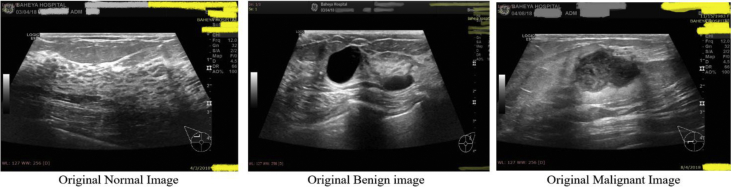
\includegraphics[width=\columnwidth]{figs/busi_real_cases.jpg}
\caption{Representative original breast ultrasound scans from the BUSI collection: normal, benign, and malignant cases. Reproduced from Al-Dhabyani et al.~\cite{aldhabyani2020busi}, Figure 2, under CC BY 4.0. These images are not part of our experiments.}
\label{fig:busi}
\end{figure}

\paragraph{Contributions.}
(i) We implement, in plain NumPy, logistic regression by stochastic gradient ascent (SGA), a Dirichlet evidential head with a verified analytic gradient, and a random-Fourier-feature (RFF) variant, and combine them with entropy rejection and quantile threshold calibration.
(ii) We evaluate them against RBF-SVM, boosted trees and a bootstrap ensemble on three datasets, with a random-rejection control, risk--coverage analysis, calibration, out-of-distribution (OOD) detection, and controlled flips of minority-class labels in both training and calibration data.
(iii) We report where the published benefits reproduce (relative error reduction under rejection, benefit of evidential uncertainty for OOD detection with bounded features) and where they do not (robustness from regularisation, benefit of $u$ for error ranking, calibration gains), with paired tests over seeds.
All code, tables and MLflow logs are provided with the source.

% =====================================================================
\section{Related work}
\paragraph{Selective classification.} Chow~\cite{chow1970reject} formalised the error--reject trade-off; Geifman and El-Yaniv~\cite{geifman2017selective} introduced risk--coverage analysis for deep networks. Aperstein et al.~\cite{aperstein2026selective} apply a post-hoc, per-label entropy threshold with quantile calibration to a frozen multi-label DenseNet-121, reporting balanced-accuracy gains of $+0.07$ to $+0.09$ at 70\% coverage on NIH ChestX-ray14 and showing that entropy matches Monte Carlo dropout and ensembles at lower cost.
\paragraph{Evidential learning.} Sensoy et al.~\cite{sensoy2018edl} predict Dirichlet parameters from non-negative evidence; the uncertainty mass is $u=K/S$ in the subjective-logic formulation~\cite{josang2016subjective,han2021tmc}. UIOS~\cite{wang2023uios} uses evidential uncertainty and validation-selected thresholds for open-set retinal screening, reporting classification and anomaly-detection metrics. MedFormer-UR~\cite{sibhai2026medformerur} applies evidential uncertainty per token to gate feature refinement in a vision transformer and reports ECE, Brier score, and NLL. BEDL~\cite{tchokponhoue2026bedl} combines evidential outputs with Bayesian weights and finds that the relative performance of the methods varies across datasets and uncertainty measures.
\paragraph{Label noise.} Surveys~\cite{frenay2014noise} and theory~\cite{natarajan2013noisy} show that noisy labels degrade flexible models more, and that loss and regularisation choices matter. We test that expectation for selective prediction specifically.

% =====================================================================
\section{Methods}
Let $x\in\mathbb{R}^d$ be a feature vector, $y\in\{0,\dots,K-1\}$ a label, and $\hat p(x)\in\Delta^{K-1}$ a predictive distribution with $\hat y=\arg\max_k \hat p_k$. Data are first split 60/20/20 into train, calibration pool and test sets (stratified); the calibration pool is then split equally into a probability-calibration subset and a disjoint rejection-threshold subset. Class $k$ gets weight $w_k=\sqrt{n_{\max}/n_k}$ in every training loss, following~\cite{aperstein2026selective}. Figure~\ref{fig:pipe} summarises the pipeline.

\begin{figure*}[t]
\centering
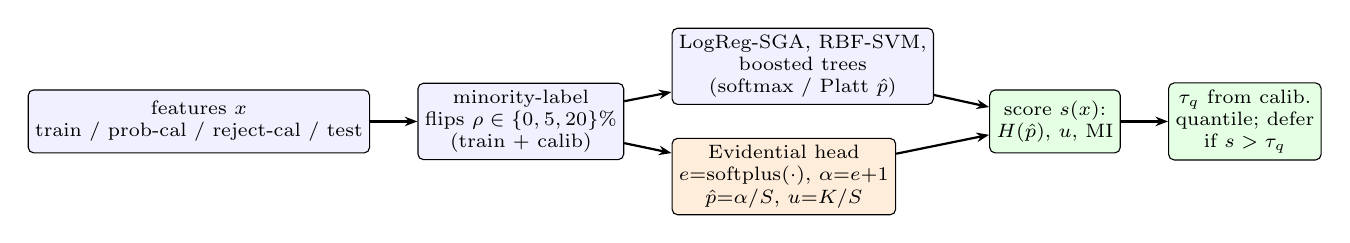
\begin{tikzpicture}[font=\scriptsize, node distance=5mm and 6mm,
  box/.style={draw, rounded corners=2pt, align=center, minimum height=8mm, inner sep=2.5pt, fill=blue!6},
  ebox/.style={draw, rounded corners=2pt, align=center, minimum height=8mm, inner sep=2.5pt, fill=orange!14},
  sbox/.style={draw, rounded corners=2pt, align=center, minimum height=8mm, inner sep=2.5pt, fill=green!10},
  arr/.style={-{Stealth[length=1.6mm]}, thick}]
\node[box] (data) {features $x$\\train / prob-cal / reject-cal / test};
\node[box, right=of data] (noise) {minority-label\\flips $\rho\in\{0,5,20\}\%$\\(train + calib)};
\node[box, right=of noise, yshift=7mm] (base) {LogReg-SGA, RBF-SVM,\\boosted trees\\(softmax / Platt $\hat p$)};
\node[ebox, right=of noise, yshift=-7mm] (edl) {Evidential head\\$e{=}\mathrm{softplus}(\cdot)$, $\alpha{=}e{+}1$\\$\hat p{=}\alpha/S$, $u{=}K/S$};
\node[sbox, right=of base, xshift=1mm, yshift=-7mm] (score) {score $s(x)$:\\$H(\hat p)$, $u$, MI};
\node[sbox, right=of score] (thr) {$\tau_q$ from calib.\\quantile; defer\\if $s>\tau_q$};
\draw[arr] (data)--(noise); \draw[arr] (noise)--(base); \draw[arr] (noise)--(edl);
\draw[arr] (base)--(score); \draw[arr] (edl)--(score); \draw[arr] (score)--(thr);
\end{tikzpicture}
\caption{Pipeline. Borrowed mechanisms are shaded: evidential head (orange) from~\cite{sensoy2018edl,wang2023uios}; entropy score and quantile-calibrated deferral (green) from~\cite{aperstein2026selective}. Test labels are never perturbed.}
\label{fig:pipe}
\end{figure*}

\subsection{Base classifiers}
\textbf{LogReg-SGA.} For the binary case, mini-batch stochastic gradient \emph{ascent} on the weighted, $\ell_2$-penalised log-likelihood updates
\begin{equation}
\theta \leftarrow \theta + \eta_t\Big(\tfrac1{|\mathcal B|}\textstyle\sum_{i\in\mathcal B} w_{y_i}\,\big(y_i-\sigma(\theta^\top x_i+b)\big)\,x_i-\lambda\theta\Big),
\end{equation}
with batch size 32, $\eta_0{=}0.05$ decayed per epoch, 30 epochs. The sigmoid gives $P(y{=}1\mid x)$; the multiclass version replaces $\sigma$ by a softmax. We use $\lambda=10^{-4}$ (base) and $\lambda=0.05$ (robust variant).
\textbf{RBF-SVM} ($C{=}1$ base, $C{=}0.1$ robust) and the linear SVM produce probabilities through Platt scaling~\cite{platt1999probabilistic}, fitted on the probability-calibration subset. The disjoint rejection-threshold subset is used to select $\tau_q$. In noisy runs, both subsets have independently corrupted labels. \textbf{Boosted trees} use 100 depth-3 trees (learning rate 0.1) as base and 60 depth-2 trees (rate 0.05, subsample 0.7, min leaf 10) as robust variant. Gaussian Naive Bayes, KNN ($k{=}15$), a depth-5 CART tree and AdaBoost complete the Phase~I--II baselines (scikit-learn~\cite{pedregosa2011sklearn}).

\subsection{Evidential heads}
Following~\cite{sensoy2018edl,wang2023uios}, a head outputs non-negative evidence $e=\mathrm{softplus}(W\phi(x)+b)\in\mathbb{R}_{\ge0}^K$, Dirichlet parameters $\alpha=e+1$ and strength $S=\sum_k\alpha_k$, giving
\begin{equation}
\hat p_k=\alpha_k/S,\qquad u=K/S .
\end{equation}
Training minimises the expected cross-entropy under the Dirichlet plus an annealed KL regulariser that shrinks evidence for wrong classes:
\begin{equation}
\begin{aligned}
\mathcal L_i &= w_{y_i}\Big[\sum_k y_{ik}\big(\psi(S_i)-\psi(\alpha_{ik})\big)\\
&\qquad +\lambda_t\,\mathrm{KL}\big(\mathrm{Dir}(\tilde\alpha_i)\,\|\,\mathrm{Dir}(\mathbf 1)\big)\Big],\\
\tilde\alpha_i &= y_i+(\mathbf 1-y_i)\odot\alpha_i,
\end{aligned}
\end{equation}
with $\lambda_t=0.1\min(1,t/10)$ and $\psi$ the digamma function. We derived the gradient analytically (it matches finite differences to $10^{-10}$) and optimise with Adam~\cite{kingma2015adam} (100 epochs, batch 64). \textbf{EDL-Linear} takes $\phi(x)=x$; its decision boundary is linear but $\hat p$ is not a logistic function of the score. \textbf{EDL-RFF} uses $\phi(x)=\cos(\Omega^\top x+\beta)$ with 300 random Fourier features~\cite{rahimi2007random} approximating an RBF kernel ($\gamma=1/d$), giving a bounded, non-linear feature map. We do not use UIOS's temperature cross-entropy term. As an epistemic baseline in the spirit of BEDL's Monte Carlo comparators, \textbf{Ens-LogReg} averages 20 bootstrap LogReg-SGA models; its mutual information is $\mathrm{MI}=H(\bar p)-\frac1B\sum_b H(p_b)$.

\subsection{Selective prediction}
Three uncertainty scores are used (higher means less certain): entropy $H(\hat p)=-\sum_k\hat p_k\log_2\hat p_k$, evidential mass $u$, and MI. For operational thresholding, following~\cite{aperstein2026selective}, $\tau_q$ is the $q$-quantile of scores among correctly classified calibration samples; test samples with $s(x)>\tau_q$ are deferred. This calibration rule conditions on calibration correctness, so its threshold depends on the classifier's performance and on the observed calibration labels (which are corrupted in the noisy-label experiments). The induced test coverage is therefore not fixed and is reported as such. Separately, to compare ranking quality at a common target, we fix test coverage $c$ by deferring the $1-c$ highest-scoring test samples. This is an evaluation at imposed coverage, not an operational threshold calibrated without test labels. We report balanced accuracy (macro recall) of the retained set, $\BA_c$; relative balanced-error reduction $\Delta\mathrm{BER}=(\mathrm{BE}_{1}-\mathrm{BE}_{0.7})/\mathrm{BE}_{1}$ with $\mathrm{BE}=1-\BA$; and AURC$=\frac1{|G|}\sum_{c\in G}(1-\BA_c)$ over $G=\{0.70,0.75,\dots,1.0\}$ (lower is better). A \emph{random-rejection control} defers the same fraction at random. ECE uses 15 equal-width bins on top-label confidence.

\subsection{Label noise protocol}
For a rate $\rho\in\{5\%,20\%\}$ we flip that fraction of minority-class labels (to another class chosen uniformly) in the training \emph{and} calibration splits, since both come from the same annotated pool; test labels stay clean. The ``robust variants'' above change only regularisation or tree capacity.

% =====================================================================
\section{Experimental setup}
\textbf{Dataset A (real).} Breast Cancer Wisconsin (Diagnostic)~\cite{street1993wisconsin}: all 357 benign cases and 63 randomly drawn malignant cases (15\% minority) per seed. We use the 10 ``standard-error'' features, because with all 30 features the task is nearly saturated (AUC $\approx0.997$) and leaves no room to see rejection effects. The test set has 84 cases ($\approx$13 malignant), so single-seed results are noisy; we use 20 seeds. \textbf{Dataset B (synthetic).} \texttt{make\_classification}, $n{=}10{,}000$, $d{=}40$ (10 informative, 5 redundant), 8\% minority, 2\% random label noise; the dataset is fixed and seeds change splits and model randomness (10 seeds). \textbf{Dataset C (multiclass).} A synthetic 3-class set ($n{=}6{,}000$, $d{=}30$, proportions 17/62/21\%) loosely inspired by the imbalance of breast-ultrasound benchmarks (10 seeds). Because A is a hand-chosen real subset and B, C are synthetic, our numbers are not comparable in absolute terms to image-based studies.

\textbf{Statistics and tracking.} Tables give means over seeds; where ``$\pm$'' appears it is the standard deviation across seeds. Paired two-sided Wilcoxon signed-rank tests are used across seeds. The six primary comparisons use Holm-adjusted $p$-values; other tests are exploratory and uncorrected. With 10 seeds the smallest attainable exact two-sided value is 0.002. The Task~3.2 runs (baseline versus robust variants, $\rho\in\{0,5\%\}$) are logged to MLflow~\cite{zaharia2018mlflow} with hyper-parameters, precision, recall, F1 and the fitted model as an artifact (14 runs). All hyper-parameters were fixed a priori and not tuned on test data.

% =====================================================================
\section{Results}
\subsection{Baselines and decision boundaries}
Table~\ref{tab:base} shows that on the larger set B the three strongest classifiers by balanced accuracy are gradient boosting (0.901), RBF-SVM (0.891) and logistic regression (0.868); these three are the ones retrained under noise. On the small real set A the ranking is flatter (BA 0.74--0.82; boosting 0.819, logistic regression 0.801, RBF-SVM 0.761), with the linear SVM the best by PR-AUC (0.850). The PR curve is the more informative view at 8--15\% prevalence~\cite{saito2015prc} (Fig.~\ref{fig:bnd}d): ROC curves differ little (c), while PR-AUC separates SVM/boosting (0.88) from LogReg (0.83). Fig.~\ref{fig:bnd}a--b contrasts a linear boundary (LogReg) with the axis-aligned staircase of a depth-5 tree on a 2-D PCA projection of A.

\begin{table*}[t]
\centering\caption{Clean-label baselines (mean $\pm$ s.d. over seeds). F1 is for the minority class; BA is balanced accuracy.}\label{tab:base}
\footnotesize\resizebox{\textwidth}{!}{\begin{tabular}{lcccccccc}\toprule
 & \multicolumn{4}{c}{Dataset A (Wisconsin, real)} & \multicolumn{4}{c}{Dataset B (synthetic)}\\
\cmidrule(lr){2-5}\cmidrule(lr){6-9}
Model & F1 & BA & ROC-AUC & PR-AUC & F1 & BA & ROC-AUC & PR-AUC\\\midrule
LogReg (SGA) & 0.67\,{\scriptsize$\pm$0.10} & 0.801\,{\scriptsize$\pm$0.061} & 0.923\,{\scriptsize$\pm$0.033} & 0.771\,{\scriptsize$\pm$0.074} & 0.77\,{\scriptsize$\pm$0.01} & 0.868\,{\scriptsize$\pm$0.008} & 0.926\,{\scriptsize$\pm$0.009} & 0.827\,{\scriptsize$\pm$0.015}\\
Naive Bayes & 0.65\,{\scriptsize$\pm$0.11} & 0.779\,{\scriptsize$\pm$0.065} & 0.902\,{\scriptsize$\pm$0.052} & 0.764\,{\scriptsize$\pm$0.097} & 0.65\,{\scriptsize$\pm$0.01} & 0.835\,{\scriptsize$\pm$0.006} & 0.918\,{\scriptsize$\pm$0.011} & 0.724\,{\scriptsize$\pm$0.011}\\
KNN ($k$=15) & 0.64\,{\scriptsize$\pm$0.10} & 0.743\,{\scriptsize$\pm$0.055} & 0.908\,{\scriptsize$\pm$0.042} & 0.766\,{\scriptsize$\pm$0.078} & 0.54\,{\scriptsize$\pm$0.03} & 0.686\,{\scriptsize$\pm$0.016} & 0.918\,{\scriptsize$\pm$0.013} & 0.781\,{\scriptsize$\pm$0.022}\\
Decision tree (d=5) & 0.63\,{\scriptsize$\pm$0.09} & 0.786\,{\scriptsize$\pm$0.061} & 0.788\,{\scriptsize$\pm$0.071} & 0.509\,{\scriptsize$\pm$0.108} & 0.70\,{\scriptsize$\pm$0.03} & 0.829\,{\scriptsize$\pm$0.019} & 0.860\,{\scriptsize$\pm$0.018} & 0.648\,{\scriptsize$\pm$0.034}\\
AdaBoost & 0.68\,{\scriptsize$\pm$0.10} & 0.803\,{\scriptsize$\pm$0.064} & 0.914\,{\scriptsize$\pm$0.041} & 0.770\,{\scriptsize$\pm$0.080} & 0.73\,{\scriptsize$\pm$0.02} & 0.860\,{\scriptsize$\pm$0.015} & 0.928\,{\scriptsize$\pm$0.006} & 0.785\,{\scriptsize$\pm$0.017}\\
Gradient boosting & 0.70\,{\scriptsize$\pm$0.06} & 0.819\,{\scriptsize$\pm$0.043} & 0.916\,{\scriptsize$\pm$0.036} & 0.767\,{\scriptsize$\pm$0.086} & 0.84\,{\scriptsize$\pm$0.02} & 0.901\,{\scriptsize$\pm$0.012} & 0.953\,{\scriptsize$\pm$0.011} & 0.883\,{\scriptsize$\pm$0.018}\\
Linear SVM & 0.75\,{\scriptsize$\pm$0.07} & 0.824\,{\scriptsize$\pm$0.047} & 0.949\,{\scriptsize$\pm$0.027} & 0.850\,{\scriptsize$\pm$0.063} & 0.79\,{\scriptsize$\pm$0.02} & 0.835\,{\scriptsize$\pm$0.015} & 0.924\,{\scriptsize$\pm$0.009} & 0.829\,{\scriptsize$\pm$0.015}\\
RBF-SVM & 0.64\,{\scriptsize$\pm$0.12} & 0.761\,{\scriptsize$\pm$0.067} & 0.926\,{\scriptsize$\pm$0.028} & 0.788\,{\scriptsize$\pm$0.074} & 0.86\,{\scriptsize$\pm$0.02} & 0.894\,{\scriptsize$\pm$0.011} & 0.946\,{\scriptsize$\pm$0.013} & 0.880\,{\scriptsize$\pm$0.015}\\
\bottomrule\end{tabular}}
\end{table*}

\begin{figure*}[t]
\centering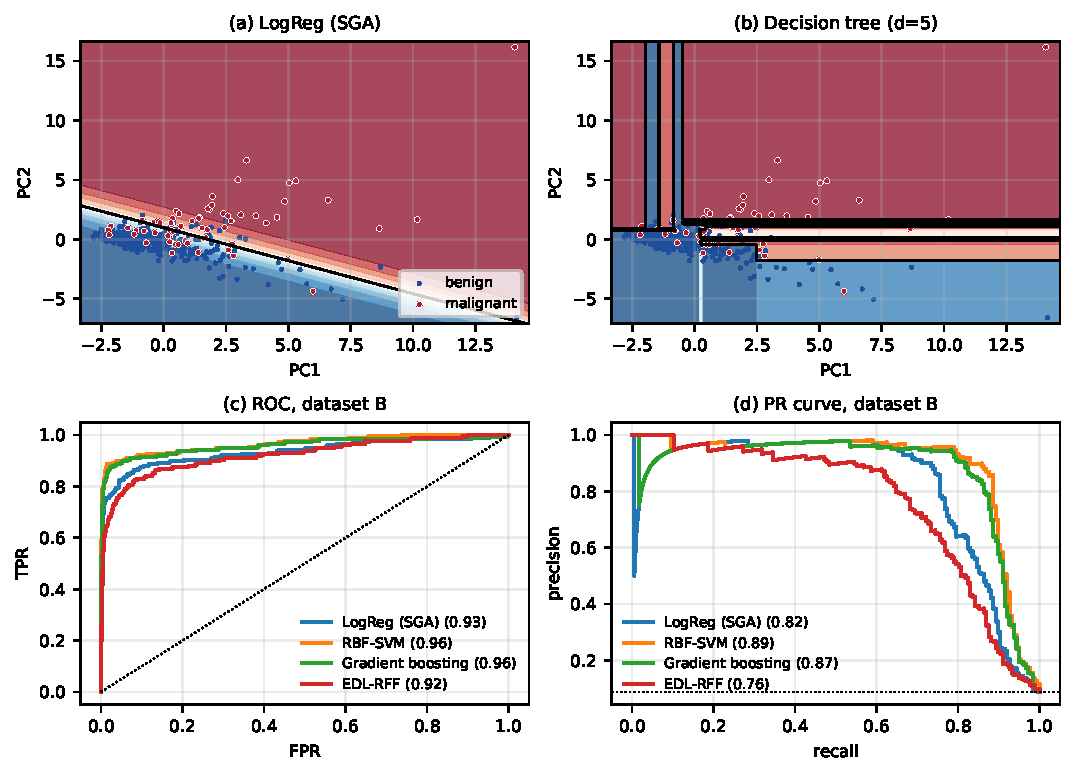
\includegraphics[width=0.92\textwidth]{figs/boundaries_prc.pdf}
\caption{(a,b) Decision boundaries of LogReg-SGA and a depth-5 decision tree on the first two principal components of dataset A (contour: $p{=}0.5$). (c,d) Illustrative ROC and precision--recall curves on dataset B for seed 0; legends give AUC and average precision. These single-seed curves are not the seed-aggregated results reported in tables.}\label{fig:bnd}
\end{figure*}

\subsection{Selective prediction with clean labels}
Table~\ref{tab:sel} gives the main result. At 70\% imposed test coverage, entropy rejection raises balanced accuracy in the reported clean-label configurations on both datasets. On B, the gain over full coverage is $+0.058$ for LogReg ($\Delta$BER 44\%), $+0.032$ for boosting (32\%), $+0.026$ for RBF-SVM (24\%) and $+0.051$ for EDL-Linear (38\%); on A the gains range from $+0.056$ to $+0.115$ ($\Delta$BER 29--59\%). Table~\ref{tab:coverage} reports balanced accuracy at 50\%, 70\%, and 90\% coverage and AURC for the three principal classical models, matching operating points used in selective-prediction studies. Across-seed paired 95\% intervals for the entropy-versus-random difference are positive for all six dataset/model combinations; all six Wilcoxon comparisons remain below 0.05 after Holm correction (Table~\ref{tab:infer}). These intervals describe variability across repeated runs and do not quantify uncertainty over independent cohorts. Fig.~\ref{fig:rc} shows the aggregated risk--coverage curves. Figure~\ref{fig:thr} illustrates operational thresholding: for LogReg on B, $q=0.70$ yields test coverage 0.69 ($\BA=0.926$) and $q=0.90$ coverage 0.88 ($\BA=0.908$). These are distinct evaluations: one applies calibration-derived thresholds, while the coverage tables fix coverage directly using test scores.

\begin{table*}[t]
\centering\caption{Selective prediction with clean labels at 70\% imposed coverage (mean over seeds; best BA$_{0.7}$ and AURC per dataset in bold). $\Delta$BER: relative balanced-error reduction. H: entropy; $u$: evidential mass; MI: ensemble mutual information.}\label{tab:sel}
\scriptsize\resizebox{\textwidth}{!}{\begin{tabular}{lccccc|ccccc}\toprule
 & \multicolumn{5}{c}{Dataset A (Wisconsin, real)} & \multicolumn{5}{c}{Dataset B (synthetic)}\\
Model + score & BA$_{1.0}$ & BA$_{0.7}$ & $\Delta$BER & AURC & ECE & BA$_{1.0}$ & BA$_{0.7}$ & $\Delta$BER & AURC & ECE\\\midrule
LogReg-SGA + entropy & 0.801 & 0.916 & 54\% & 0.140 & 0.130 & 0.868 & 0.926 & 44\% & 0.094 & 0.044\\
RBF-SVM + entropy & 0.761 & 0.832 & 27\% & 0.206 & 0.068 & 0.894 & 0.920 & 24\% & 0.085 & 0.011\\
GradBoost + entropy & 0.819 & 0.875 & 29\% & 0.150 & 0.075 & 0.901 & \textbf{0.933} & 32\% & \textbf{0.073} & 0.033\\
LogReg ensemble (H) & 0.801 & 0.915 & 55\% & 0.139 & 0.141 & 0.869 & 0.924 & 42\% & 0.094 & 0.047\\
LogReg ensemble (MI) & 0.801 & 0.848 & 23\% & 0.175 & 0.141 & 0.869 & 0.919 & 39\% & 0.099 & 0.047\\
EDL-Linear (H) & 0.812 & 0.926 & 59\% & \textbf{0.131} & 0.133 & 0.866 & 0.917 & 38\% & 0.099 & 0.072\\
EDL-Linear ($u$) & 0.812 & \textbf{0.926} & 65\% & 0.134 & 0.133 & 0.866 & 0.903 & 28\% & 0.112 & 0.072\\
EDL-RFF (H) & 0.810 & 0.897 & 46\% & 0.147 & 0.070 & 0.854 & 0.886 & 22\% & 0.117 & 0.058\\
EDL-RFF ($u$) & 0.810 & 0.849 & 24\% & 0.163 & 0.070 & 0.854 & 0.863 & 6\% & 0.136 & 0.058\\
\bottomrule\end{tabular}}
\end{table*}

\begin{table*}[t]
\centering\caption{Balanced accuracy at several fixed test coverages and AURC for the three principal entropy-based classifiers (mean $\pm$ s.d. across seeds).}\label{tab:coverage}
\small\begin{tabular}{llcccc}\toprule
Dataset & Model & BA @50\% & BA @70\% & BA @90\% & AURC$\downarrow$\\\midrule
Dataset A & Logistic regression & 0.962\,{\scriptsize$\pm$0.058} & 0.916\,{\scriptsize$\pm$0.056} & 0.841\,{\scriptsize$\pm$0.062} & 0.140\,{\scriptsize$\pm$0.053}\\
Dataset A & RBF-SVM & 0.874\,{\scriptsize$\pm$0.181} & 0.832\,{\scriptsize$\pm$0.111} & 0.782\,{\scriptsize$\pm$0.083} & 0.206\,{\scriptsize$\pm$0.076}\\
Dataset A & Gradient boosting & 0.865\,{\scriptsize$\pm$0.180} & 0.875\,{\scriptsize$\pm$0.082} & 0.849\,{\scriptsize$\pm$0.051} & 0.150\,{\scriptsize$\pm$0.051}\\
Dataset B & Logistic regression & 0.936\,{\scriptsize$\pm$0.013} & 0.926\,{\scriptsize$\pm$0.012} & 0.905\,{\scriptsize$\pm$0.008} & 0.094\,{\scriptsize$\pm$0.008}\\
Dataset B & RBF-SVM & 0.927\,{\scriptsize$\pm$0.032} & 0.920\,{\scriptsize$\pm$0.020} & 0.916\,{\scriptsize$\pm$0.014} & 0.085\,{\scriptsize$\pm$0.013}\\
Dataset B & Gradient boosting & 0.943\,{\scriptsize$\pm$0.020} & 0.933\,{\scriptsize$\pm$0.016} & 0.931\,{\scriptsize$\pm$0.010} & 0.073\,{\scriptsize$\pm$0.012}\\
\bottomrule\end{tabular}
\end{table*}

\begin{table*}[t]
\centering\caption{Primary paired comparison of entropy rejection with random rejection at 70\% coverage. $\Delta$BA is entropy minus random; intervals are paired 95\% Student-$t$ intervals across seeds. Holm adjustment is applied to this six-test family.}\label{tab:infer}
\small\begin{tabular}{llccc}\toprule
Dataset & Model & Mean $\Delta$BA & 95\% CI & Holm $p$\\\midrule
A (real tabular) & Logistic regression & +0.117 & [+0.085, +0.149] & 0.00016\\
A (real tabular) & RBF-SVM & +0.071 & [+0.020, +0.121] & 0.0136\\
A (real tabular) & Gradient boosting & +0.059 & [+0.022, +0.096] & 0.0117\\
B (synthetic) & Logistic regression & +0.057 & [+0.050, +0.065] & 0.00977\\
B (synthetic) & RBF-SVM & +0.025 & [+0.012, +0.038] & 0.0117\\
B (synthetic) & Gradient boosting & +0.031 & [+0.023, +0.039] & 0.00977\\
\bottomrule\end{tabular}
\end{table*}

\begin{figure*}[t]
\centering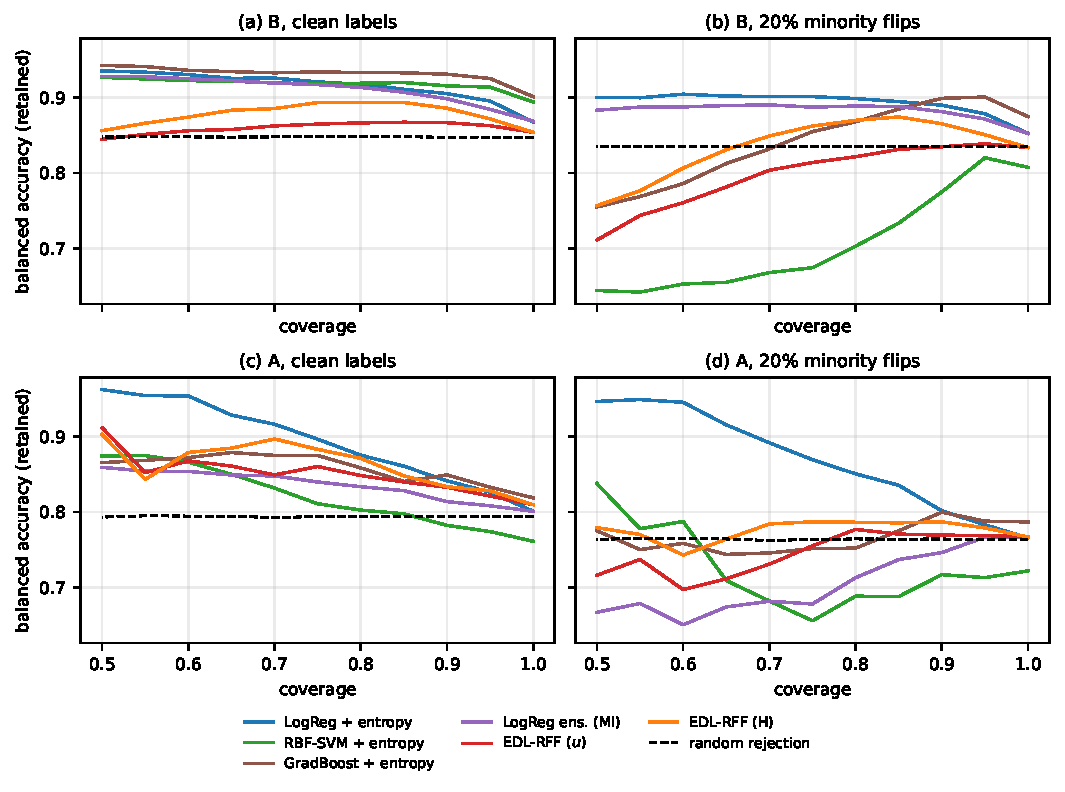
\includegraphics[width=0.92\textwidth]{figs/risk_coverage.pdf}
\caption{Balanced accuracy of the retained set versus coverage (mean over seeds). Panels are arranged in a 2$\times$2 grid: synthetic B (clean, 20\% flips) on top; real tabular A (clean, 20\% flips) below.}\label{fig:rc}
\end{figure*}

\paragraph{Evidential uncertainty versus entropy.} The evidential mass $u$ was \emph{not} a better error-ranking signal than entropy. On B, $u$ lowers $\BA_{0.7}$ relative to $H$ for EDL-Linear ($-0.014$, $p=0.006$) and EDL-RFF ($-0.023$, $p=0.014$); on A the same holds for EDL-RFF ($-0.048$, $p=0.002$) and shows no difference for EDL-Linear ($p=0.80$). The same pattern appears in the 3-class set (Table~\ref{tab:multi}). This is expected: $u=K/S$ measures the \emph{total evidence}, whereas misclassifications mostly occur where evidence for two classes is high and similar, which entropy captures. EDL itself neither helps nor hurts accuracy here: EDL-Linear matches LogReg on B (BA 0.866 vs.\ 0.868, $p=0.43$) and is slightly higher on A (0.812 vs.\ 0.801, $p=0.17$). Its ECE is higher than LogReg's (0.072 vs.\ 0.044 on B), so the calibration gain reported for evidential routing in MedFormer-UR (ECE 0.184$\to$0.069, the best of 15 values of its routing strength in a single table~\cite{sibhai2026medformerur}) is not reproduced here, although that intervention differs from ours.
\paragraph{Calibration metrics.} Table~\ref{tab:calibration} adds Brier score and negative log-likelihood (NLL), which complement ECE and are reported alongside it in medical-image calibration studies. All three are computed on clean test labels; lower is better. The ECE uses 15 equal-width bins, so it is sensitive to binning and should not be read as a complete calibration assessment. The evidential variants share the same predictive probabilities between their $H$ and $u$ rows, so their probability-calibration metrics are identical.

\begin{table*}[t]
\centering\caption{Test-set probability-calibration metrics (mean $\pm$ s.d. over seeds; lower is better). ECE uses 15 equal-width bins.}\label{tab:calibration}
\scriptsize\begin{tabular}{lccc|ccc}\toprule
 & \multicolumn{3}{c}{Dataset A} & \multicolumn{3}{c}{Dataset B}\\
Model + score & ECE$\downarrow$ & Brier$\downarrow$ & NLL$\downarrow$ & ECE$\downarrow$ & Brier$\downarrow$ & NLL$\downarrow$\\\midrule
LogReg-SGA + entropy & 0.130\,{\scriptsize$\pm$0.024} & 0.174\,{\scriptsize$\pm$0.031} & 0.312\,{\scriptsize$\pm$0.039} & 0.044\,{\scriptsize$\pm$0.003} & 0.073\,{\scriptsize$\pm$0.003} & 0.154\,{\scriptsize$\pm$0.005}\\
RBF-SVM + entropy & 0.068\,{\scriptsize$\pm$0.022} & 0.147\,{\scriptsize$\pm$0.037} & 0.403\,{\scriptsize$\pm$0.426} & 0.011\,{\scriptsize$\pm$0.004} & 0.041\,{\scriptsize$\pm$0.003} & 0.096\,{\scriptsize$\pm$0.008}\\
GradBoost + entropy & 0.075\,{\scriptsize$\pm$0.020} & 0.149\,{\scriptsize$\pm$0.036} & 0.314\,{\scriptsize$\pm$0.094} & 0.033\,{\scriptsize$\pm$0.003} & 0.047\,{\scriptsize$\pm$0.004} & 0.108\,{\scriptsize$\pm$0.007}\\
LogReg ensemble (H) & 0.141\,{\scriptsize$\pm$0.022} & 0.188\,{\scriptsize$\pm$0.031} & 0.334\,{\scriptsize$\pm$0.036} & 0.047\,{\scriptsize$\pm$0.004} & 0.073\,{\scriptsize$\pm$0.003} & 0.154\,{\scriptsize$\pm$0.005}\\
LogReg ensemble (MI) & 0.141\,{\scriptsize$\pm$0.022} & 0.188\,{\scriptsize$\pm$0.031} & 0.334\,{\scriptsize$\pm$0.036} & 0.047\,{\scriptsize$\pm$0.004} & 0.073\,{\scriptsize$\pm$0.003} & 0.154\,{\scriptsize$\pm$0.005}\\
EDL-Linear (H) & 0.133\,{\scriptsize$\pm$0.025} & 0.189\,{\scriptsize$\pm$0.031} & 0.334\,{\scriptsize$\pm$0.035} & 0.072\,{\scriptsize$\pm$0.003} & 0.078\,{\scriptsize$\pm$0.003} & 0.173\,{\scriptsize$\pm$0.004}\\
EDL-Linear ($u$) & 0.133\,{\scriptsize$\pm$0.025} & 0.189\,{\scriptsize$\pm$0.031} & 0.334\,{\scriptsize$\pm$0.035} & 0.072\,{\scriptsize$\pm$0.003} & 0.078\,{\scriptsize$\pm$0.003} & 0.173\,{\scriptsize$\pm$0.004}\\
EDL-RFF (H) & 0.070\,{\scriptsize$\pm$0.016} & 0.151\,{\scriptsize$\pm$0.028} & 0.260\,{\scriptsize$\pm$0.040} & 0.058\,{\scriptsize$\pm$0.004} & 0.089\,{\scriptsize$\pm$0.009} & 0.183\,{\scriptsize$\pm$0.013}\\
EDL-RFF ($u$) & 0.070\,{\scriptsize$\pm$0.016} & 0.151\,{\scriptsize$\pm$0.028} & 0.260\,{\scriptsize$\pm$0.040} & 0.058\,{\scriptsize$\pm$0.004} & 0.089\,{\scriptsize$\pm$0.009} & 0.183\,{\scriptsize$\pm$0.013}\\
\bottomrule\end{tabular}
\end{table*}

\begin{figure}[t]
\centering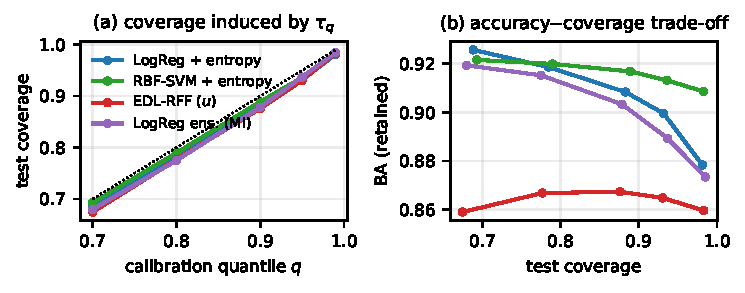
\includegraphics[width=\columnwidth]{figs/threshold.pdf}
\caption{Threshold sensitivity on dataset B (clean): the calibration quantile $q\in\{0.70,\dots,0.99\}$ controls the induced coverage (a) and the accuracy--coverage trade-off (b).}\label{fig:thr}
\end{figure}

\subsection{Robustness to minority-label noise (Task 3.2)}
Table~\ref{tab:noise} compares each baseline with its ``robust'' variant. Three observations stand out. \emph{First}, stronger regularisation did not improve final balanced accuracy: on B the robust LogReg is worse than the base model at every noise level and loses more balanced accuracy at 20\% (drop 0.027 vs.\ 0.015); the lower-capacity boosted trees lose similar amounts (0.025 vs.\ 0.026) from a lower starting point; the SVM with $C{=}0.1$ has a smaller drop (0.077 vs.\ 0.087) but nearly identical final BA (0.808 vs.\ 0.808), within seed variability. \emph{Second}, RBF-SVM is the most noise-sensitive evaluated model on B (drop 0.087), while LogReg and EDL-Linear are the least (drop 0.014--0.015). On A at 20\% noise, EDL-Linear has the best BA of the evaluated models (0.805 vs.\ 0.765 for LogReg, $p=0.024$ uncorrected; drop 0.008 vs.\ 0.035), but with about 13 positive test cases this result is suggestive. \emph{Third}, the \emph{rejection gain} changes sign for two evaluated models: with 20\% minority-label flips, deferring 30\% lowers balanced accuracy of RBF-SVM by 0.140 and boosting by 0.043 on B ($p\le0.004$ versus random rejection), while LogReg and EDL-Linear retain gains of $+0.049$ and $+0.039$. A plausible but untested explanation is that these models fit flipped minority points and become confidently wrong there, while correctly classified minority cases near the boundary are deferred. Platt scaling is fitted on a separate but also label-corrupted calibration subset. This interaction is consistent with the caveat in~\cite{aperstein2026selective}; it does not establish a general property of all flexible classifiers.

\begin{table*}[t]
\centering\caption{Effect of minority-label flips (mean over seeds; drop = BA clean $-$ BA at 20\%; rejection gain = $\BA_{0.7}-\BA_{1.0}$ at 20\% noise, entropy score).}\label{tab:noise}
\footnotesize\resizebox{\textwidth}{!}{\begin{tabular}{lccccc}\toprule
Model & BA clean & BA 5\% & BA 20\% & drop (20\%) & rejection gain (20\%)\\\midrule
\multicolumn{6}{l}{\textit{Dataset B}}\\
LogReg (SGA), $\lambda{=}10^{-4}$ & 0.868 & 0.865 & 0.853 & 0.015\,{\scriptsize$\pm$0.007} & +0.049\\
LogReg (SGA), $\lambda{=}0.05$ & 0.848 & 0.845 & 0.822 & 0.027\,{\scriptsize$\pm$0.006} & +0.019\\
RBF-SVM, $C{=}1$ & 0.894 & 0.876 & 0.808 & 0.087\,{\scriptsize$\pm$0.013} & $-$0.140\\
RBF-SVM, $C{=}0.1$ & 0.885 & 0.874 & 0.808 & 0.077\,{\scriptsize$\pm$0.016} & $-$0.123\\
Boosted trees, depth 3 & 0.901 & 0.893 & \textbf{0.875} & 0.026\,{\scriptsize$\pm$0.011} & $-$0.043\\
Boosted trees, depth 2 + shrinkage & 0.834 & 0.827 & 0.809 & 0.025\,{\scriptsize$\pm$0.011} & $-$0.096\\
EDL-Linear & 0.866 & 0.864 & 0.853 & 0.014\,{\scriptsize$\pm$0.006} & +0.039\\
EDL-RFF & 0.854 & 0.852 & 0.834 & 0.020\,{\scriptsize$\pm$0.013} & +0.015\\
\midrule
\multicolumn{6}{l}{\textit{Dataset A}}\\
LogReg (SGA), $\lambda{=}10^{-4}$ & 0.801 & 0.796 & 0.765 & 0.035\,{\scriptsize$\pm$0.041} & +0.126\\
LogReg (SGA), $\lambda{=}0.05$ & 0.797 & 0.785 & 0.754 & 0.042\,{\scriptsize$\pm$0.044} & +0.127\\
RBF-SVM, $C{=}1$ & 0.761 & 0.718 & 0.722 & 0.039\,{\scriptsize$\pm$0.045} & $-$0.040\\
RBF-SVM, $C{=}0.1$ & 0.758 & 0.719 & 0.717 & 0.040\,{\scriptsize$\pm$0.053} & +0.018\\
Boosted trees, depth 3 & 0.819 & 0.813 & 0.787 & 0.032\,{\scriptsize$\pm$0.054} & $-$0.041\\
Boosted trees, depth 2 + shrinkage & 0.829 & 0.822 & 0.791 & 0.037\,{\scriptsize$\pm$0.035} & $-$0.073\\
EDL-Linear & 0.812 & 0.813 & \textbf{0.805} & 0.008\,{\scriptsize$\pm$0.047} & +0.118\\
EDL-RFF & 0.810 & 0.801 & 0.767 & 0.043\,{\scriptsize$\pm$0.043} & +0.017\\

\bottomrule\end{tabular}}
\end{table*}

\subsection{Out-of-distribution detection}
UIOS and BEDL motivate evidential uncertainty mainly through OOD detection. We test two shifts on the clean-trained models: \emph{far-OOD} inputs $x\sim\mathcal N(0,3^2I)$ (standardised space) and a \emph{covariate shift} $x'=1.5x+\mu$ with $\mu_j=\pm1$. Table~\ref{tab:ood} reports the AUROC of separating OOD from in-distribution test data. The results are sharply split by feature map. \textbf{Linear models are worse than chance} (AUROC 0.28--0.37 for far-OOD): far from the data the logits grow, so both entropy \emph{and} the linear evidential mass become more confident, analogous to the over-confident predictions far from the training data that BEDL~\cite{tchokponhoue2026bedl} attributes, citing Hein et al., to ReLU networks. \textbf{With bounded RFF features, $u$ works:} EDL-RFF reaches 0.89 (B) and 0.95 (A) on far-OOD, above its own entropy (0.83 and 0.88; gains $+0.057$ and $+0.074$, $p=0.002$), so the qualitative advantage of evidential over entropy-based scores reported in UIOS is reproduced. Against the RBF-SVM with Platt-scaled entropy, EDL-RFF is worse on B (0.89 vs.\ 0.96, $p=0.002$) and better on A far-OOD (0.95 vs.\ 0.91, $p=0.049$), with no difference under the milder shift on A ($p=0.38$). The bootstrap-ensemble MI is also far better than ensemble entropy (0.52 vs.\ 0.33 on B far-OOD), but remains weak because linear members extrapolate in the same direction.

\begin{table*}[t]
\centering\caption{OOD detection AUROC (mean $\pm$ s.d. over 10 seeds); 0.5 is chance.}\label{tab:ood}
\footnotesize\resizebox{\textwidth}{!}{\begin{tabular}{lcccc}\toprule
 & \multicolumn{2}{c}{Dataset B} & \multicolumn{2}{c}{Dataset A}\\
\cmidrule(lr){2-3}\cmidrule(lr){4-5}
Model + score & far-OOD & shift & far-OOD & shift\\\midrule
LogReg + entropy & 0.28\,{\scriptsize$\pm$0.01} & 0.45\,{\scriptsize$\pm$0.20} & 0.35\,{\scriptsize$\pm$0.04} & 0.41\,{\scriptsize$\pm$0.10}\\
EDL-Linear (H) & 0.35\,{\scriptsize$\pm$0.01} & 0.48\,{\scriptsize$\pm$0.18} & 0.37\,{\scriptsize$\pm$0.07} & 0.42\,{\scriptsize$\pm$0.09}\\
EDL-Linear ($u$) & 0.33\,{\scriptsize$\pm$0.01} & 0.47\,{\scriptsize$\pm$0.20} & 0.32\,{\scriptsize$\pm$0.05} & 0.38\,{\scriptsize$\pm$0.16}\\
LogReg ensemble (H) & 0.33\,{\scriptsize$\pm$0.01} & 0.48\,{\scriptsize$\pm$0.20} & 0.37\,{\scriptsize$\pm$0.04} & 0.42\,{\scriptsize$\pm$0.10}\\
LogReg ensemble (MI) & 0.52\,{\scriptsize$\pm$0.02} & 0.63\,{\scriptsize$\pm$0.22} & 0.81\,{\scriptsize$\pm$0.04} & 0.77\,{\scriptsize$\pm$0.08}\\
GradBoost + entropy & 0.68\,{\scriptsize$\pm$0.03} & 0.70\,{\scriptsize$\pm$0.06} & 0.69\,{\scriptsize$\pm$0.05} & 0.53\,{\scriptsize$\pm$0.17}\\
RBF-SVM + entropy & 0.96\,{\scriptsize$\pm$0.01} & 0.92\,{\scriptsize$\pm$0.03} & 0.91\,{\scriptsize$\pm$0.05} & 0.75\,{\scriptsize$\pm$0.06}\\
EDL-RFF (H) & 0.83\,{\scriptsize$\pm$0.02} & 0.80\,{\scriptsize$\pm$0.02} & 0.87\,{\scriptsize$\pm$0.03} & 0.72\,{\scriptsize$\pm$0.07}\\
EDL-RFF ($u$) & 0.89\,{\scriptsize$\pm$0.03} & 0.85\,{\scriptsize$\pm$0.04} & 0.95\,{\scriptsize$\pm$0.02} & 0.77\,{\scriptsize$\pm$0.08}\\
\bottomrule\end{tabular}}
\end{table*}

\subsection{Multiclass setting}
Table~\ref{tab:multi} repeats the analysis with softmax LogReg-SGA, boosting and evidential heads on the 3-class set. Gradient boosting is best (accuracy 0.946, BA 0.925); entropy rejection at 70\% coverage raises BA by 0.04--0.08 for all models ($\Delta$BER 44--55\% with entropy). Rejection by $u$ is markedly weaker (EDL-Linear: 12\% vs.\ 44\% with entropy), consistent with the binary results. With 20\% minority-label noise the models lose between 0.004 (EDL-Linear) and 0.026 (boosting) BA; the multiclass gap between entropy and $u$ persists.

\begin{table*}[t]
\centering\caption{Three-class results (mean $\pm$ s.d. over 10 seeds). BA is macro recall.}\label{tab:multi}
\scriptsize\resizebox{\textwidth}{!}{\begin{tabular}{lcccccc}\toprule
Model + score & Acc & BA$_{1.0}$ & BA$_{0.7}$ & $\Delta$BER & ECE$\downarrow$ & BA$_{1.0}$ (20\% noise)\\\midrule
Softmax LogReg (SGA) + entropy & 0.907\,{\scriptsize$\pm$0.009} & 0.880\,{\scriptsize$\pm$0.010} & 0.937\,{\scriptsize$\pm$0.011} & 48\% & 0.034\,{\scriptsize$\pm$0.008} & 0.874\,{\scriptsize$\pm$0.010}\\
Softmax LogReg, $\lambda$=0.05 & 0.907\,{\scriptsize$\pm$0.010} & 0.876\,{\scriptsize$\pm$0.012} & 0.930\,{\scriptsize$\pm$0.009} & 44\% & 0.110\,{\scriptsize$\pm$0.011} & 0.865\,{\scriptsize$\pm$0.010}\\
Gradient boosting + entropy & 0.946\,{\scriptsize$\pm$0.006} & 0.925\,{\scriptsize$\pm$0.010} & 0.966\,{\scriptsize$\pm$0.006} & 55\% & 0.044\,{\scriptsize$\pm$0.008} & 0.899\,{\scriptsize$\pm$0.011}\\
LogReg ensemble (H) & 0.907\,{\scriptsize$\pm$0.008} & 0.879\,{\scriptsize$\pm$0.009} & 0.939\,{\scriptsize$\pm$0.010} & 49\% & 0.036\,{\scriptsize$\pm$0.008} & 0.872\,{\scriptsize$\pm$0.011}\\
LogReg ensemble (MI) & 0.907\,{\scriptsize$\pm$0.008} & 0.879\,{\scriptsize$\pm$0.009} & 0.939\,{\scriptsize$\pm$0.011} & 50\% & 0.036\,{\scriptsize$\pm$0.008} & 0.872\,{\scriptsize$\pm$0.011}\\
EDL-Linear (H) & 0.908\,{\scriptsize$\pm$0.008} & 0.873\,{\scriptsize$\pm$0.011} & 0.929\,{\scriptsize$\pm$0.010} & 44\% & 0.141\,{\scriptsize$\pm$0.007} & 0.869\,{\scriptsize$\pm$0.010}\\
EDL-Linear ($u$) & 0.908\,{\scriptsize$\pm$0.008} & 0.873\,{\scriptsize$\pm$0.011} & 0.889\,{\scriptsize$\pm$0.012} & 12\% & 0.141\,{\scriptsize$\pm$0.007} & 0.869\,{\scriptsize$\pm$0.010}\\
EDL-RFF (H) & 0.894\,{\scriptsize$\pm$0.009} & 0.856\,{\scriptsize$\pm$0.013} & 0.935\,{\scriptsize$\pm$0.011} & 55\% & 0.106\,{\scriptsize$\pm$0.007} & 0.837\,{\scriptsize$\pm$0.012}\\
EDL-RFF ($u$) & 0.894\,{\scriptsize$\pm$0.009} & 0.856\,{\scriptsize$\pm$0.013} & 0.904\,{\scriptsize$\pm$0.014} & 34\% & 0.106\,{\scriptsize$\pm$0.007} & 0.837\,{\scriptsize$\pm$0.012}\\
\bottomrule\end{tabular}}
\end{table*}

\subsection{Context relative to published results}
The balanced-error reductions are of a similar order to those reported for chest X-rays, but differences in datasets, backbones, labels and protocols make this contextual rather than a reproduction. Our tabular results also let us test controlled label flips, an interaction that prior selective-imaging work identifies as a caveat but does not quantify~\cite{aperstein2026selective}.


% =====================================================================
\section{Discussion and limitations}
The experiments show that post-hoc entropy rejection can improve balanced accuracy at reduced coverage on the evaluated tabular and synthetic clean-label settings. The relative balanced-error reductions are of a similar order of magnitude to those reported for chest X-rays, but the tasks and protocols differ; this is a contextual comparison, not a reproduction or validation of the published image-based results. Evidential heads did not consistently improve in-distribution error ranking or ECE relative to logistic regression in our setting. EDL-RFF uncertainty outperformed its entropy score for OOD detection in the evaluated shifts, whereas the linear evidential head did not. These results are specific to the tested data and models.
\textbf{Noise.} The most practically relevant finding is that selective prediction and label noise interact: the same rejection rule that helps a regularised linear model can degrade a kernel machine or ensemble of trees. We also found no evidence that merely increasing regularisation is a remedy; noise-aware losses~\cite{natarajan2013noisy}, instance-level noise-robust training or noise-aware calibration are more promising directions.

\textbf{Limitations.} (1) The data are one small real tabular set and two synthetic sets with no images; the Wisconsin features were extracted from digitized images, but we evaluate no image pixels or image-derived backbone features. The BUSI scans in Fig.~\ref{fig:busi} are included only as clearly labelled clinical context and are not experimental data. (2) Noise is class-conditional minority-label flipping; real annotation noise may depend on instance and annotator. (3) Hyper-parameters were fixed, not tuned, and the evidential heads are simple (no temperature loss as in UIOS, no deep backbone). (4) Holm correction and paired intervals are reported for the six primary clean-label entropy-versus-random comparisons only. Other $p$-values remain exploratory and uncorrected; the intervals quantify seed variability, not independent-patient uncertainty. Dataset B's generation is fixed and dataset A has about 13 positive test cases. (5) The explanation for the negative rejection gain under noise is a hypothesis we did not test. (6) The calibration pool is divided in half for probability and threshold calibration, reducing the sample size available to estimate each stage; class-weighted training also affects probability calibration.

% =====================================================================
\section{Conclusion}
This study empirically examined whether uncertainty-estimation and selective-prediction mechanisms used in medical imaging are useful with classical classifiers under controlled minority-class label flips. On the evaluated tabular and synthetic datasets, entropy-based rejection improved balanced accuracy at 70\% imposed coverage, while random rejection did not yield comparable gains. Evidential uncertainty did not consistently improve the ranking of classification errors over entropy, although EDL-RFF uncertainty outperformed its entropy score for OOD detection in the tested settings. Rejection reduced balanced accuracy for the evaluated RBF-SVM and gradient-boosting models under 20\% minority-label flips. These observations show that rejection outcomes depend on the model and corruption protocol. The results are preliminary: no medical images or image-derived features were evaluated, only six primary comparisons received multiplicity correction, and the real dataset's test set is small. Future work should evaluate image-derived features, instance-dependent annotation noise, independent probability and threshold calibration, and corrected statistical comparisons with uncertainty intervals.

\section*{Acknowledgment}
This work was completed for Practical Work~4 on Robust Classification and Uncertainty Modeling, Department of Computer Engineering, ENSPY.

\section*{Code Availability}
Python sources (\texttt{lib.py}, \texttt{run\_experiments.py}, \texttt{run\_ood.py}, \texttt{analyze.py}, \texttt{mlflow\_run.py}), result CSVs and the MLflow database accompany this manuscript.

\IEEEtriggeratref{12}
\IEEEtriggercmd{\newpage}
\bibliographystyle{IEEEtran}
\bibliography{refs}

\end{document}
